\documentclass[italian,bachelor]{unibg}

\title{Analisi dei fattori \\bibliometrici per autori di paper scientifici}
\subtitle{Sviluppo di un software per la \\raccolta e lo studio dei dati}
\advisor{Chiar.mo Prof.\newline Stefano~Giulio~Paraboschi}
% \coadvisor{Chiar.mo Prof.~Ed Smith}

\department{Ingegneria Gestionale, dell'Informazione e della Produzione}
\course{Ingegneria Informatica}
\class{L-8}

\author{Andrea Rota}
\studentid{1054128}
\academicyear{2022/2023}

\begin{document}

% ----------------------- Default listings
\definecolor{lightbackground}{RGB}{250, 250, 250}

\lstset{
    upquote=true,
    numbers=left,
    stepnumber=1,
    frame=single,
    backgroundcolor = \color{lightbackground}
}

\maketitle
\emptypage

\begin{abstract}
Questa tesi si concentra sullo sviluppo di un'applicazione per l'acquisizione e l'analisi di dati bibliometrici sfruttando le API della piattaforma Scopus. Il progetto si articola su tre obiettivi fondamentali: la creazione di un sistema efficace per il download massivo di dati relativi ad articoli e autori da Scopus; lo sviluppo di strumenti analitici sofisticati per la manipolazione e l'analisi di tali dati, che comprendono aggregazione e interpretazione; e la realizzazione di un'interfaccia utente intuitiva, progettata per facilitare l'accesso e la navigazione attraverso diverse tipologie di analisi e relative visualizzazioni grafiche. L'intento del software è quello di rendere l'analisi bibliometrica di specifici gruppi di autori scientifici più accessibile e fruibile, ponendo le basi per ulteriori innovazioni in questo campo. In aggiunta, lo studio pone in evidenza alcune delle limitazioni del progetto attuale e propone direzioni future per il suo sviluppo e miglioramento.
\end{abstract}

\emptypage
\toc[figures,tables,listings]
\emptypage

\clearpage
\pagenumbering{arabic}

\chapter{Introduzione}
\section{Obiettivi della tesi}
Questa tesi ha come obiettivo primario lo sviluppo di un'applicazione software dedicata all'acquisizione di dati  bibliometrici, attraverso l'utilizzo di API (interfaccia di programmazione dell'applicazione), dalla piattaforma bibliografica Scopus. Il software mira, successivamente, all'analisi di tali dati, fornendo una visualizzazione grafica dei risultati semplice e intuitiva.

Nello specifico, questa tesi si propone di raggiungere tre obiettivi interconnessi:
\begin{enumerate}
    \item \textbf{Download di massa}: il primo obiettivo è la progettazione e lo sviluppo di un software in grado di accedere alla piattaforma Scopus attraverso API. Questo software sarà in grado di recuperare dati relativi agli articoli e agli autori.

    \item \textbf{Analisi dei dati}: un secondo obiettivo è l'implementazione di strumenti di analisi che consentano di elaborare e manipolare i dati bibliometrici scaricati. Ciò includerà la possibilità di aggregare e analizzare diversi indici bibliometrici e dati precedentemente raccolti.

    \item \textbf{Interfaccia utente}: la creazione di un'interfaccia utente intuitiva e accessibile rappresenta un terzo obiettivo fondamentale. L'obiettivo è fornire ai ricercatori, istituzioni accademiche e bibliotecari un'interfaccia utente che semplifichi l'accesso ai dati e agevoli la navigazione tra le diverse analisi.
\end{enumerate}
Questo lavoro punta quindi a costruire uno strumento che semplifichi l'analisi di un certo gruppo di autori scientifici e a fornire una base solida per ulteriori sviluppi in questo campo.

Tutto il codice sviluppato durante la ricerca è reso disponibile in un repository dedicato su GitHub \cite{codeBachelorThesis}. In linea con i principi di apertura e accessibilità, il codice è pubblicato sotto la licenza MIT, una scelta che riflette l'impegno verso la condivisione delle conoscenze e la facilitazione dell'uso e dell'adattamento del software da parte di altri ricercatori e sviluppatori.


\section{Importanza dell'analisi bibliometrica per autori scientifici}

La bibliometria, una branca della scientometria, utilizza metodi matematici e statistici per esaminare la distribuzione delle pubblicazioni scientifiche e valutarne l'importanza all'interno delle comunità accademiche. Questa metodologia quantitativa si avvale di indicatori bibliometrici, derivati da fonti bibliografiche affidabili, per misurare vari aspetti della ricerca scientifica, come produttività, impatto, popolarità, prestigio e capacità critica \cite{cassella2011nuovi}.

L'analisi bibliometrica offre molteplici vantaggi quando utilizzata in modo oculato. Ad esempio è uno strumento per le istituzioni accademiche, che possono sfruttarla per valutare i ricercatori e assegnare finanziamenti per la ricerca. Inoltre, aiuta i bibliotecari a individuare le riviste di riferimento da acquisire per le collezioni e fornisce un criterio per i redattori di riviste scientifiche nella selezione di revisori per le pubblicazioni. Non da ultimo, l'analisi bibliometrica rappresenta un mezzo semplice, economico ed efficace per confrontare e valutare l'attività di ricerca in vari contesti.

Gli autori scientifici, grazie ai risultati dell'analisi bibliometrica, possono:
\begin{enumerate}
  \item Valutare l'impatto del proprio lavoro di ricerca dimostrando l'originalità e la rilevanza della propria attività.
  \item Identificare i colleghi e le istituzioni che hanno contribuito in modo significativo alla propria produzione scientifica scegliendo collaborazioni scientifiche fruttuose.
  \item Selezionare le conferenze e le riviste più adatte per la pubblicazione delle proprie attività, in quanto la scelta di dove pubblicare o presenziare può aumentare la visibilità delle proprie ricerche \cite{anziliero2013bibliometria}.
\end{enumerate}

All'interno di questo lavoro verrà esaminato principalmente l'indicatore bibliometrico $h$-index (o indice di Hirsch), un indicatore bibliometrico che misura la produttività e l'impatto di un autore o di un ricercatore sulla base delle citazioni delle sue pubblicazioni scientifiche. Il calcolo dell'$h$-index avviene nel seguente modo: le pubblicazioni dell'autore vengono ordinate in ordine decrescente in base al numero di citazioni ricevute, e l'$h$-index rappresenta il numero massimo di pubblicazioni che hanno ricevuto almeno $h$ citazioni ciascuna \cite{h-index}.

A titolo di esempio, consideriamo un autore che ha pubblicato 5 articoli e che ha ricevuto rispettivamente 12, 7, 7, 4 e 2 citazioni per ciascun articolo; il suo $h$-index sarà 4, poiché almeno 4 pubblicazioni hanno ricevuto almeno 4 citazioni ciascuna.

Tuttavia, è importante notare che l'$h$-index, sebbene sia un indicatore utile, non è privo di critiche poiché, essendo un semplice numero, non fornisce sempre il quadro più completo dell'impatto del lavoro di un autore. Ad esempio può variare in base alla piattaforma bibliografica utilizzata e può essere influenzato dal fenomeno dell'autocitazionismo, sia a livello individuale che organizzativo. Inoltre, l'$h$-index potrebbe non dare il giusto riconoscimento alle pubblicazioni altamente citate \cite{h-index-problems, h-index-problems-2}.

\chapter{Applicativo per la raccolta e preparazione dei dati}\label{scopusBulkDownloader}

Nel contesto del presente lavoro si è reso necessario sviluppare un sistema dedicato all'acquisizione e preparazione di dati provenienti dalla piattaforma bibliografica Scopus, una delle più grandi banche dati di abstract e citazioni di letteratura scientifica peer-reviewed \cite{scopus-website} e successiva aggregazione con la classificazione delle conferenze informatiche \cite{conference-rating-website} redatta dall'associazione GRuppo dei professori e ricercatori in INformatica (GRIN) \cite{GRIN-website}.

\section{Progettazione e architettura}
In questo paragrafo vengono prima esaminati alcuni aspetti delle policy di Elsevier, successivamente si approfondiscono le API di Scopus illustrandone il funzionamento e i dati gestiti. Si conclude con una presentazione dell'architettura selezionata e del flusso di lavoro dell'applicativo.
\newline

Al fine di fornire una panoramica chiara e comprensibile delle decisioni architetturali adottate in questo studio è necessario delineare alcune disposizioni stipulate all'interno delle ``Elsevier Provisions for Text and Data Mining'' \cite{scopus-policy}, così come le direttive associate all'utilizzo delle chiavi di accesso alle API di Scopus \cite{scopus-key-settings}:
\begin{itemize}
    \item \textbf{Divieto di scraping}: Elsevier enuncia con precisione nei suoi termini di servizio le modalità consentite per l'accesso e l'interrogazione dei suoi contenuti attraverso le API. È espressamente proibito l'impiego di robot, spider o qualsiasi altro software automatizzato per estrarre dati dai loro portali.

    \item \textbf{Limite chiavi}: ogni utente è autorizzato a generare un massimo di dieci chiavi per interagire con le API di Elsevier.

    \item \textbf{Limite richieste}: ogni chiave individuale è soggetta a restrizioni quantificate sia in termini di richieste al secondo che settimanali, differenti a seconda del servizio specifico desiderato. Inoltre a seconda del tipo di dati voluti, potrebbero essere imposti limiti sul numero di risultati restituiti da ogni richiesta.

    \item \textbf{Rete universitaria}: l'accesso a Scopus è consentito unicamente attraverso la rete universitaria, a meno che non venga fornito un token specifico associato a una determinata chiave per l'utilizzo esterno.
\end{itemize}

Le API di Scopus adottano un'architettura REpresentational State Transfer (RESTful) \cite{scopus-api-description}, questo significa che esse forniscono una rappresentazione dello stato di una risorsa specifica, permettendo un'interazione affidabile e scalabile con i dati. Una delle principali caratteristiche di questa architettura è la capacità di rispondere a richieste in diversi formati e, in particolare, le API di Scopus supportano vari formati di risposta, tra cui \texttt{application/xml}, \texttt{application/json} e \texttt{text/html} \cite{scopus-api-specs}. Per le esigenze del presente lavoro, ci concentreremo sull'acquisizione di documenti nel formato JavaScript Object Notation (JSON), che offre una struttura dati leggibile e facilmente manipolabile per l'analisi e l'elaborazione.

Per garantire una chiara comprensione dell'organizzazione dei dati acquisiti dalla piattaforma Scopus, è essenziale delineare la struttura delle due tipologie di documenti JSON trattati nel presente lavoro: autore e abstract.
Il primo, l'autore, incapsula le informazioni relative a un ricercatore catalogato su Scopus \cite{author-scopus}; all'interno della Tabella~\ref{tab:json_structure_author} viene offerta una panoramica dettagliata, concentrandosi sugli attributi di maggiore rilievo per il presente lavoro.
\begin{table}[ht]
    \centering
    \begin{tabularx}{\textwidth}{|l|l|X|}
        \hline
        \textbf{Campo} & \textbf{Tipo di Dato} & \textbf{Descrizione} \\
        \hline
        \texttt{\_id} & Oggetto & Identificativo unico del documento \\
        \hline
        \texttt{coredata} & Oggetto & Dati identificativi dell'autore e dei suoi contributi \\
        \hline
        \texttt{h-index} & Stringa & $h$-index dell'autore \\
        \hline
        \texttt{coauthor-count} & Stringa & Numero di coautori dell'autore \\
        \hline
        \texttt{affiliation-current} & Oggetto & Affiliazione corrente dell'autore \\
        \hline
        \texttt{subject-areas} & Oggetto & Aree di specializzazione dell'autore \\
        \hline
        \texttt{author-profile} & Oggetto & Profilo dettagliato dell'autore, incluso nome, affiliazioni passate e periodo di pubblicazione  \\
        \hline
    \end{tabularx}
    \caption{Struttura JSON dell'oggetto ``Autore''}
    \label{tab:json_structure_author}
\end{table}

Il secondo, l'abstract, contiene le informazioni di una pubblicazione catalogata su Scopus \cite{abstract-scopus}. Similmente a quanto fatto per gli autori, in Tabella~\ref{tab:json_structure_abstract} sono presenti i principali campi di un abstract.

Tenendo conto dei requisiti e delle specifiche sopra menzionati, è stato concepito un sistema formato da un modulo dedicato all'interfacciamento con le API e alla successiva preparazione dei dati e un database di tipo non relazionale orientato ai documenti per la memorizzazione e gestione delle informazioni raccolte.

Per ultimo, si definisce il flusso sequenziale di lavoro dell'applicativo, ossia la sequenza di eventi necessari per scaricare e aggregare i dati:
\begin{enumerate}
    \item \textbf{Estrazione degli abstract}: download degli abstract dalle API di Scopus secondo i criteri decisi dall'utente e successivo salvataggio su database.
    \item \textbf{Estrazione degli autori}: ricerca degli identificativi degli autori all'interno degli abstract e successivo recupero delle informazioni dalle API di Scopus e archiviazione su database.
    \item \textbf{Aggregazione dei Dati}: Aggregazione degli autori e degli abstract da database con i dati presenti nella classificazione delle conferenze informatiche redatta da GRIN.
\end{enumerate}

\begin{table}[ht]
    \centering
    \begin{tabularx}{\textwidth}{|l|l|X|}
        \hline
        \textbf{Campo} & \textbf{Tipo di Dato} & \textbf{Descrizione} \\
        \hline
        \texttt{\_id} & Oggetto & Identificativo unico dell'abstract nella forma di un ObjectId. \\
        \hline
        \texttt{title} & Stringa & Titolo dell'abstract o dell'articolo. \\
        \hline
        \texttt{subtype} & Stringa & Codice per il sottotipo dell'articolo. \\
        \hline
        \texttt{affilname} & Stringa & Nome dell'istituzione affiliata. \\
        \hline
        \texttt{affiliation\_city} & Stringa & Città dell'istituzione affiliata. \\
        \hline
        \texttt{affiliation\_country} & Stringa & Paese dell'istituzione affiliata. \\
        \hline
        \texttt{author\_count} & Stringa & Numero totale di autori dell'articolo. \\
        \hline
        \texttt{author\_ids} & Stringa & Elenco degli ID degli autori su Scopus separati da ``;'', il primo è l'autore principale. \\
        \hline
        \texttt{coverDate} & Stringa & Data di pubblicazione dell'articolo. \\
        \hline
        \texttt{publicationName} & Stringa & Nome della pubblicazione o della rivista. \\
        \hline
        \texttt{aggregationType} & Stringa & Tipo di aggregazione (es. rivista, conferenza, ecc.). \\
        \hline
        \texttt{description} & Stringa & Descrizione o sommario dell'articolo. \\
        \hline
        \texttt{citedby\_count} & Numero & Numero di citazioni dell'articolo. \\
        \hline
    \end{tabularx}
    \caption{Struttura JSON dell'oggetto ``Abstract''}
    \label{tab:json_structure_abstract}
\end{table}

\section{Strumenti e tecnologie utilizzate}\label{scopusBulkDownloader-tech}
Si è deciso di sviluppare il modulo preposto all'interfacciamento con le API e alla successiva preparazione dei dati utilizzando Python \cite{python}, un linguaggio di programmazione ad alto livello ampiamente utilizzato per lo sviluppo di applicazioni web, scripting, analisi dati e intelligenza artificiale.
Mentre, riguardo alla selezione del sistema di gestione del database, la scelta è ricaduta su MongoDB \cite{mongodb-github}, un Database Management System (DBMS) non relazionale orientato ai documenti che archivia le informazioni in documenti BSON, una rappresentazione binaria del noto formato JSON. Questa peculiarità conferisce a MongoDB una notevole flessibilità, permettendo di adattare e modificare lo schema dei dati senza la rigidità strutturale tipica dei database relazionali. Nell'ambito di questo progetto, l'adozione di questa tecnologia è stata motivata principalmente da due fattori chiave: la sua capacità di gestire ampie quantità di dati e la sua conformità ai modelli orientati ai documenti; tale natura si è rivelata particolarmente aderente alle esigenze del nostro contesto, in cui i dati provenienti dalla piattaforma Scopus richiedono una certa versatilità nella loro elaborazione e archiviazione.

Uno degli strumenti chiave impiegati per costruire l'applicativo è Pybliometrics \cite{ROSE2019100263, pybliometrics-github}, una libreria Python specificamente progettata per l'interazione con le API di Scopus. Questa libreria facilita notevolmente il processo di acquisizione dei dati bibliometrici in base ai criteri specificati occupandosi della gestione delle chiavi multiple e dei limiti di richieste al secondo.

Per la manipolazione e aggregazione dei dati è stato fatto ricorso, attraverso l'uso delle API progettate per Python, ad Apache Spark \cite{spark-github}, un motore distribuito di elaborazione dati open source per grandi dataset che offre prestazioni elevate e supporta un'ampia varietà di operazioni analitiche.

Invece, per la gestione e il salvataggio dei dati, si è fatto uso di PyMongo \cite{pymongo-github}, un driver Python per MongoDB che permette di interagire con il database non relazionale, garantendo operazioni di lettura e scrittura efficienti e un modello di dati flessibile, adattandosi perfettamente alle esigenze del progetto.

Infine, sono state utilizzate in maniera minore Pandas \cite{pandas-github}, uno degli strumenti più potenti e flessibili disponibili per l'analisi e la manipolazione dei dati in Python e la libreria Python-dotenv \cite{python-dotenv-github} per la gestione delle variabili d'ambiente.

In sintesi, l'applicativo sfrutta una combinazione di librerie Python per scaricare, manipolare e aggregare dati da Scopus, e memorizzare i risultati in un database MongoDB. Queste tecnologie e strumenti sono stati scelti per la loro affidabilità, efficienza e facilità d'uso nel contesto della raccolta e dell'analisi dei dati.

\section{Aggregazione dei dati}
L'aggregazione dei dati riveste un ruolo cruciale nell'intero processo: una preparazione adeguata e accurata della collezione di documenti non solo semplifica, ma arricchisce e potenzia la successiva fase di analisi.

Una componente chiave di questo processo è la classificazione delle conferenze informatiche fornita da GRIN e, per fornire un quadro chiaro all'interno della Tabella~\ref{tab:example_conference_data} viene presentato un estratto del documento in formato CSV utilizzato. Questo file è delimitato dal carattere ``;'' e contiene due colonne principali: il titolo della conferenza e e la corrispondente valutazione; la classificazione GRIN prevede sette livelli, elencati in ordine decrescente: A++, A+, A, A-, B, B-, C.

\begin{table}[ht]
    \centering
    \begin{tabularx}{\textwidth}{|X|l|}
        \hline
        \textbf{Title} & \textbf{GGS Rating} \\
        \hline
        CONFERENCE ON ARTIFICIAL INTELLIGENCE & A++ \\
        \hline
        ASIAN CONFERENCE ON COMPUTER VISION & B \\
        \hline
        ACM SYMPOSIUM ON APPLIED COMPUTING & A- \\
        \hline
    \end{tabularx}
    \caption{Classificazione delle conferenze: un esempio di dati}
    \label{tab:example_conference_data}
\end{table}

L'algoritmo di aggregazione dei dati, implementato nella classe $AggregateDocuments$, si articola in quattro fasi principali, ciascuna con una funzione specifica:

\begin{enumerate}
  \item \textbf{Conversione dei tipi di dati}: alcuni campi, come \texttt{h-index} e \texttt{coauthor-count} per gli autori e \texttt{author\_count} per gli abstract, vengono convertiti da stringhe a interi semplificando le successive operazioni di analisi.
  
  \item \textbf{Correlazione con la classificazione delle conferenze}: per associare gli abstract alla classificazione delle conferenze informatiche fornita da GRIN, l'algoritmo realizza una left-join tra gli abstract e il file CSV aggiungendo ai primi un campo \texttt{GGS\_Rating} contenente il livello di rating come illustrato nel Codice~\ref{lst:script_aggregateDocuments}.
  
  \item \textbf{Aggregazione abstract per autore}: ogni autore viene associato ai propri abstract distinguendo tra quelli in cui è l'autore principale e quelli in cui è coautore. Questa distinzione è resa possibile grazie all'aggiunta di un campo \texttt{articles} che include le due liste di articoli: \texttt{main\_author} e \texttt{coauthor}.
  
  \item \textbf{Salvataggio dei dati aggregati}: una volta completate le operazioni di aggregazione, i dati risultanti vengono archiviati in una nuova collezione MongoDB denominata ``collectionAuthorsAggregate''.
\end{enumerate}

\begin{lstfloat}
    \begin{lstlisting}[
    language=Python,
    caption={Script Python per l'associazione dei rating delle conferenze},
    label={lst:script_aggregateDocuments},
    breaklines=true,
    postbreak=\mbox{\textcolor{red}{$\hookrightarrow$}\space}
    ]
def join_conference_rating(self, spark, spark_abstracts):
    spark_conferences = spark \
        .read \
        .options(delimiter=';', header=True) \
        .csv(self.FILENAME_CONFERENCE_RATING)
    
    spark_conferences = spark_conferences \
        .filter(spark_conferences['GGS Rating'] != 'Work in Progress') \
        .withColumnRenamed('GGS Rating','GGS_Rating') \
        .withColumn('Title', lower(spark_conferences.Title))

    spark_abstracts = spark_abstracts \
        .withColumn(
            'publicationName',
            lower(spark_abstracts.publicationName)
        )

    spark_join = spark_abstracts \
        .alias('abstracts') \
        .join(
            spark_conferences.alias('conferences'),
            col('publicationName') \
                .contains(spark_conferences.Title),
            'left'
        )
    
    return spark_join \
        .selectExpr('abstracts.*', 'conferences.GGS_Rating')
    \end{lstlisting}
\end{lstfloat}
\section{Interfaccia utente}
L'interfaccia utente permette agli utenti di attivare l'applicativo specificando alcuni parametri attraverso riga di comando: è possibile definire il tipo di azione da eseguire, modificare alcuni parametri e applicare dei filtri; per un'esaustiva definizione degli argomenti si rimanda alla Tabella~\ref{tab:parameters_scopusBulkDownloader}, per un esempio di comando si rimanda al Codice~\ref{lst:command_scopusBulkDownloader}.

\begin{table}[ht]
    \centering
    \begin{tabularx}{\textwidth}{|l|X|l|}
        \hline
        \textbf{Parametro} & \textbf{Descrizione} & \textbf{Valore Predefinito} \\
        \hline
        \texttt{-h, -{}-help} & Mostra la lista di tutti i comandi & - \\
        \hline
        \texttt{-{}-type} & Specifica l'azione da eseguire: & - \\
        & \texttt{aut}, scarica gli autori & \\
        & \texttt{abs}, scarica gli abstract & \\
        & \texttt{agg}, aggrega i dati & \\
        \hline
        \texttt{-{}-urimongo} & URI di MongoDB & \texttt{mongodb://localhost:27017/} \\
        \hline
        \texttt{-{}-subjarea} & Valido con \texttt{abs}, codice dell'area tematica desiderata & \texttt{COMP} \\
        \hline
        \texttt{-{}-start} & Valido con \texttt{abs}, indica l'anno di inizio da cui scaricare  & \texttt{1850} \\
        \hline
        \texttt{-{}-end} & Valido con \texttt{abs}, indica l'anno di fine da cui scaricare & \texttt{2007} \\
        \hline
    \end{tabularx}
    \caption{Parametri del comando \texttt{scopusBulkDownloader}}
    \label{tab:parameters_scopusBulkDownloader}
\end{table}

\begin{lstfloat}
    \begin{lstlisting}[basicstyle=\ttfamily, caption={Comando per scaricare gli abstract dal 2010 al 2021}, label={lst:command_scopusBulkDownloader}]
scopusBulkDownloader --type abs --start 2010 --end 2021
    \end{lstlisting}
\end{lstfloat}


\section{Limitazioni delle tecnologie utilizzate}
La necessità di analizzare un vasto insieme di autori e abstract si è scontrata con le restrizioni stabilite da Elsevier \cite{scopus-key-settings}. In particolare, le API consentono di scaricare un massimo di 5.000 autori per chiave, il che si traduce in un tetto massimo di 50.000 oggetti a settimana e questo limite, unito alla restrizione di tre richieste al secondo, esaurisce in circa cinque ore di download la quota settimanale disponibile.

Per quanto concerne gli abstract, le condizioni sono leggermente più permissive poiché il limite settimanale è fissato a 20.000 richieste, con una frequenza massima di nove al secondo e ogni singola interrogazione può recuperare fino a 25 abstract. Sebbene le restrizioni sugli autori precludano l'analisi di un vasto numero di essi, le limitazioni sugli abstract si traducono in lunghi periodi di download esclusivamente nel caso di volumi di dati particolarmente elevati.

Un'ulteriore complicazione deriva dalla necessità di effettuare questi download all'interno della rete universitaria dal momento che Elsevier fornisce un unico token, associato a una singola chiave, per ogni progetto. Di conseguenza, nel caso in cui vi sia la necessità di scaricare grandi quantità di dati, non è possibile procedere al di fuori dell'infrastruttura universitaria.
\chapter{Sviluppo del software di analisi}
La realizzazione di un software dedicato all'analisi dei dati bibliometrici è al centro di questo capitolo. Attraverso una combinazione di tecnologie, il software mira a fornire agli utenti gli strumenti necessari per esplorare, analizzare e visualizzare le analisi sui fattori bibliometrici degli autori di paper scientifici.
Nel corso di questo capitolo verrà esplorata l'architettura del software, gli strumenti e le tecnologie utilizzate, le analisi e i grafici implementati.

\section{Architettura client/server}
Le esigenze di analisi complesse, la necessità di una visualizzazione chiara e interattiva dei dati e l'importanza di condividere facilmente gli output con altri utenti hanno reso imperativo l'adozione di un'architettura robusta e flessibile per il software di analisi dei dati, l'architettura client/server si è rivelata la scelta ideale per soddisfare queste esigenze.

Nel presente contesto, il server svolge un ruolo cruciale nell'elaborazione delle richieste, eseguendo analisi dettagliate e restituendo i risultati pertinenti al client. Gestisce anche in modo efficiente l'interazione con il database MongoDB e mette a disposizione un servizio API RESTful, facilitando l'accesso e la manipolazione dei dati. Parallelamente, il client invia richieste specifiche al backend per ottenere o eseguire determinate analisi e, una volta ricevute, presenta i risultati attraverso un'interfaccia utente interattiva, garantendo che gli utenti possano comprendere e interpretare le informazioni in modo chiaro e intuitivo.

\section{Strumenti e tecnologie utilizzate}
Nel processo di sviluppo del software, particolare attenzione è stata posta nella scelta delle tecnologie e degli strumenti. Per il componente di backend la scelta del linguaggio Python è stata naturale considerando sia la volontà di mantenere una coerenza con il modulo di download e aggregazione dei dati descritto nel Capitolo~\ref{scopusBulkDownloader}, sia la sua vasta gamma di librerie dedicate all'analisi dei dati. Per accelerare lo sviluppo e garantire un'implementazione solida dell'infrastruttura web, è stato adottato Flask \cite{flask-github}, un micro framework web noto per la sua semplicità e efficienza.

Per il frontend, invece, la scelta è ricaduta su TypeScript \cite{typescript}, un linguaggio open source che estende JavaScript introducendo la tipizzazione statica. La decisione di utilizzare React \cite{react-github} come libreria per la costruzione delle interfacce utente è stata guidata dalla sua capacità di offrire un'esperienza utente fluida e reattiva, oltre alla sua popolarità e alla vasta comunità di supporto. Un'altra libreria utilizzata di fondamentale importanza è Apache ECharts \cite{apache-echarts-github}, una soluzione open source dedicata alla visualizzazione dei dati, sviluppata per creare grafici e diagrammi interattivi per il web mantenuta da Apache Software Foundation.

All'interno del lavoro sono state integrate altre librerie per semplificare lo sviluppo e potenziare le funzionalità del software, tra queste c'è Mui \cite{mui-github}, un framework UI per React basato sul Material Design \cite{material-design} di Google che ha giocato un ruolo chiave nella realizzazione di un'interfaccia grafica intuitiva e reattiva. Sul lato backend, Pandas e PyMongo sono stati essenziali per l'elaborazione, l'analisi e la gestione dei dati, queste librerie sono già state approfondite nel Paragrafo~\ref{scopusBulkDownloader-tech}.

Data la complessità e l'eterogeneità delle tecnologie impiegate in questo progetto, l'adozione di Docker \cite{docker} è stata una scelta strategica per garantire una gestione fluida e centralizzata delle numerose dipendenze. L'uso dei container ha permesso di incapsulare ogni componente del sistema in ambienti isolati, facilitando così non solo l'installazione, ma anche l'aggiornamento e la manutenzione, assicurando che ogni parte del software operi in condizioni ottimali e coerenti. Questo approccio ha inoltre contribuito a rendere il sistema più robusto e resiliente, minimizzando i rischi legati a possibili incompatibilità o conflitti tra le diverse librerie e servizi utilizzati.


\section{Funzionalità di analisi dei dati}
Il backend del progetto implementa sei diverse funzionalità di analisi dei dati, che sono:
\begin{enumerate}
    \item \textbf{Variazione media dei coautori nel tempo}: questa funzione calcola come varia il numero medio di coautori negli anni successivi all'inizio della carriera di un autore, considerando autori con un $h$-index superiore a una certa soglia decisa dall'utente.

    \item \textbf{Impatto del numero di coautori sulle citazioni}: valuta la relazione tra il numero di coautori di un articolo e il numero di citazioni che quest'ultimo ha ricevuto.

    \item \textbf{Analisi del momento di pubblicazione di articoli influenti sull'$h$-index}: definisce in quale momento della carriera di un autore sono stati pubblicati gli articoli che influenzano l'$h$-index normalizzando il risultato tra 0 (inizio carriera) e 1 (fine carriera). Nel Codice~\ref{lst:analyze_hindex_influential_articles_timing} vi è la porzione che illustra il processo di calcolo del momento di pubblicazione e relativa normalizzazione.
    Considera esclusivamente autori con un $h$-index superiore a una certa soglia decisa dall'utente.

    \item \textbf{Correlazione tra $h$-index e articoli esclusi}: cerca una correlazione tra il valore di $h$-index di un autore e il numero di articoli che non sono considerati nel calcolo di quest'indice, considerando esclusivamente autori con un $h$-index superiore a una certa soglia decisa dall'utente.

    \item \textbf{Correlazione tra $h$-index e durata della carriera}: esplora la relazione tra l'$h$-index di un autore e la durata della sua carriera.

    \item \textbf{Impatto del ranking di una conferenza sul numero di citazioni}: esamina se esiste una correlazione tra il numero di citazioni ricevute da un articolo e il ranking della conferenza in cui è stato presentato, considera esclusivamente autori con un $h$-index superiore a una certa soglia decisa dall'utente.

\end{enumerate}

\begin{lstfloat}
    \begin{lstlisting}[
    language=Python,
    caption={Calcolo del momento di pubblicazione e normalizzazione},
    label={lst:analyze_hindex_influential_articles_timing},
    breaklines=true,
    postbreak=\mbox{\textcolor{red}{$\hookrightarrow$}\space}
    ]
df_abstracts = df_abstracts \
    .sort_values('citedby_count', ascending=False) \
    .head(h_index)

df_abstracts['years_since_career_start'] = pd \
    .to_datetime(df_abstracts['coverDate']) \
    .dt.year - career_start_year

max_difference = career_end_year - career_start_year

df_abstracts['coefficient'] = \
    df_abstracts['years_since_career_start'] / max_difference
    
return df_abstracts['coefficient'].mean()
    \end{lstlisting}
\end{lstfloat}

Ognuna delle analisi sopra descritte è accessibile tramite specifici endpoint API RESTful, descritti in Tabella~\ref{table:api_endpoints}, progettati per fornire al client risposte in formato JSON, facilitando così la richiesta e la rappresentazione dei risultati.

\begin{table}[ht]
    \centering
    \begin{tabularx}{\textwidth}{|X|l|l|}
        \hline
        \textbf{Endpoint} & \textbf{Parametri} & \textbf{Valore default} \\
        \hline
        \url{/api/saved\_analyses} & - & - \\
        \hline
        \url{/api/all\_analyses} & \texttt{h-index}, \texttt{title} & 0, ``\texttt{analysis-0-hindex}'' \\
        \hline
        \url{/api/average\_coauthors\_variation\_after\_years} & \texttt{h-index} & 0 \\
        \hline
        \url{/api/coauthors\_impact\_on\_citations\_and\_hindex} & - & - \\
        \hline
        \url{/api/analyze\_hindex\_influential\_articles\_timing} & \texttt{h-index} & 0 \\
        \hline
        \url{/api/correlation\_between\_hindex\_and\_excluded\_articles} & \texttt{h-index} & 0 \\
        \hline
        \url{/api/correlation_between_hindex_and_career_duration} & - & - \\
        \hline
        \url{/api/citation\_count\_based\_on\_conference\_ranking} & \texttt{h-index} & 0 \\
        \hline
    \end{tabularx}
    \caption{Elenco degli endpoint API RESTful}
    \label{table:api_endpoints}
\end{table}

La struttura della risposta ha un campo principale contenente il risultato scalare dell'analisi e un campo \texttt{data} contenente una lista di valori o di coppie di dati utilizzati per il calcolo del campo principale; nel Codice~\ref{lst:example_json_response} è riportato un esempio di risposta.

\begin{lstfloat}
    \begin{lstlisting}[
    basicstyle=\ttfamily,
    caption={Esempio di risposta JSON di un'analisi},
    label={lst:example_json_response},
    ]
{
    "correlation": -0.06749014708602911,
    "data": [
        {
            "years_since_career_start": 0,
            "coauthors_count": 3.25
        },
        {
            "years_since_career_start": 1, 
            "coauthors_count": 4.6470588235
        },
        {
            "years_since_career_start": 2,
            "coauthors_count": 2.25
        },
        ...
    ]
}
    \end{lstlisting}
\end{lstfloat}

Quando viene invocata la funzione dell'endpoint \texttt{all\_analyses}, il sistema salva automaticamente i risultati delle analisi in una collezione MongoDB chiamata ``cacheAnalysis'' identificandoli tramite un nome e il valore di $h$-index scelto. Questa metodologia permette di accedere e visualizzare le elaborazioni passate in modo veloce e efficiente, eliminando la necessità di riprocessare i dati ad ogni nuova interrogazione.

\section{Dashboard}
Per facilitare la visualizzazione e la manipolazione dei dati analitici, è stata sviluppata una dashboard articolata in due sezioni principali. La prima offre agli utenti la possibilità di consultare e scaricare le interrogazioni precedenti, nonché di iniziare nuove analisi inserendo parametri specifici come il nome e l'$h$-index di soglia minima. La seconda sezione, invece, è dedicata alla rappresentazione dei risultati attraverso l'impiego di grafici. La Figura~\ref{fig:dashboard} illustra l'aspetto finale di questa interfaccia.

\begin{figure}[ht]
    \centering
    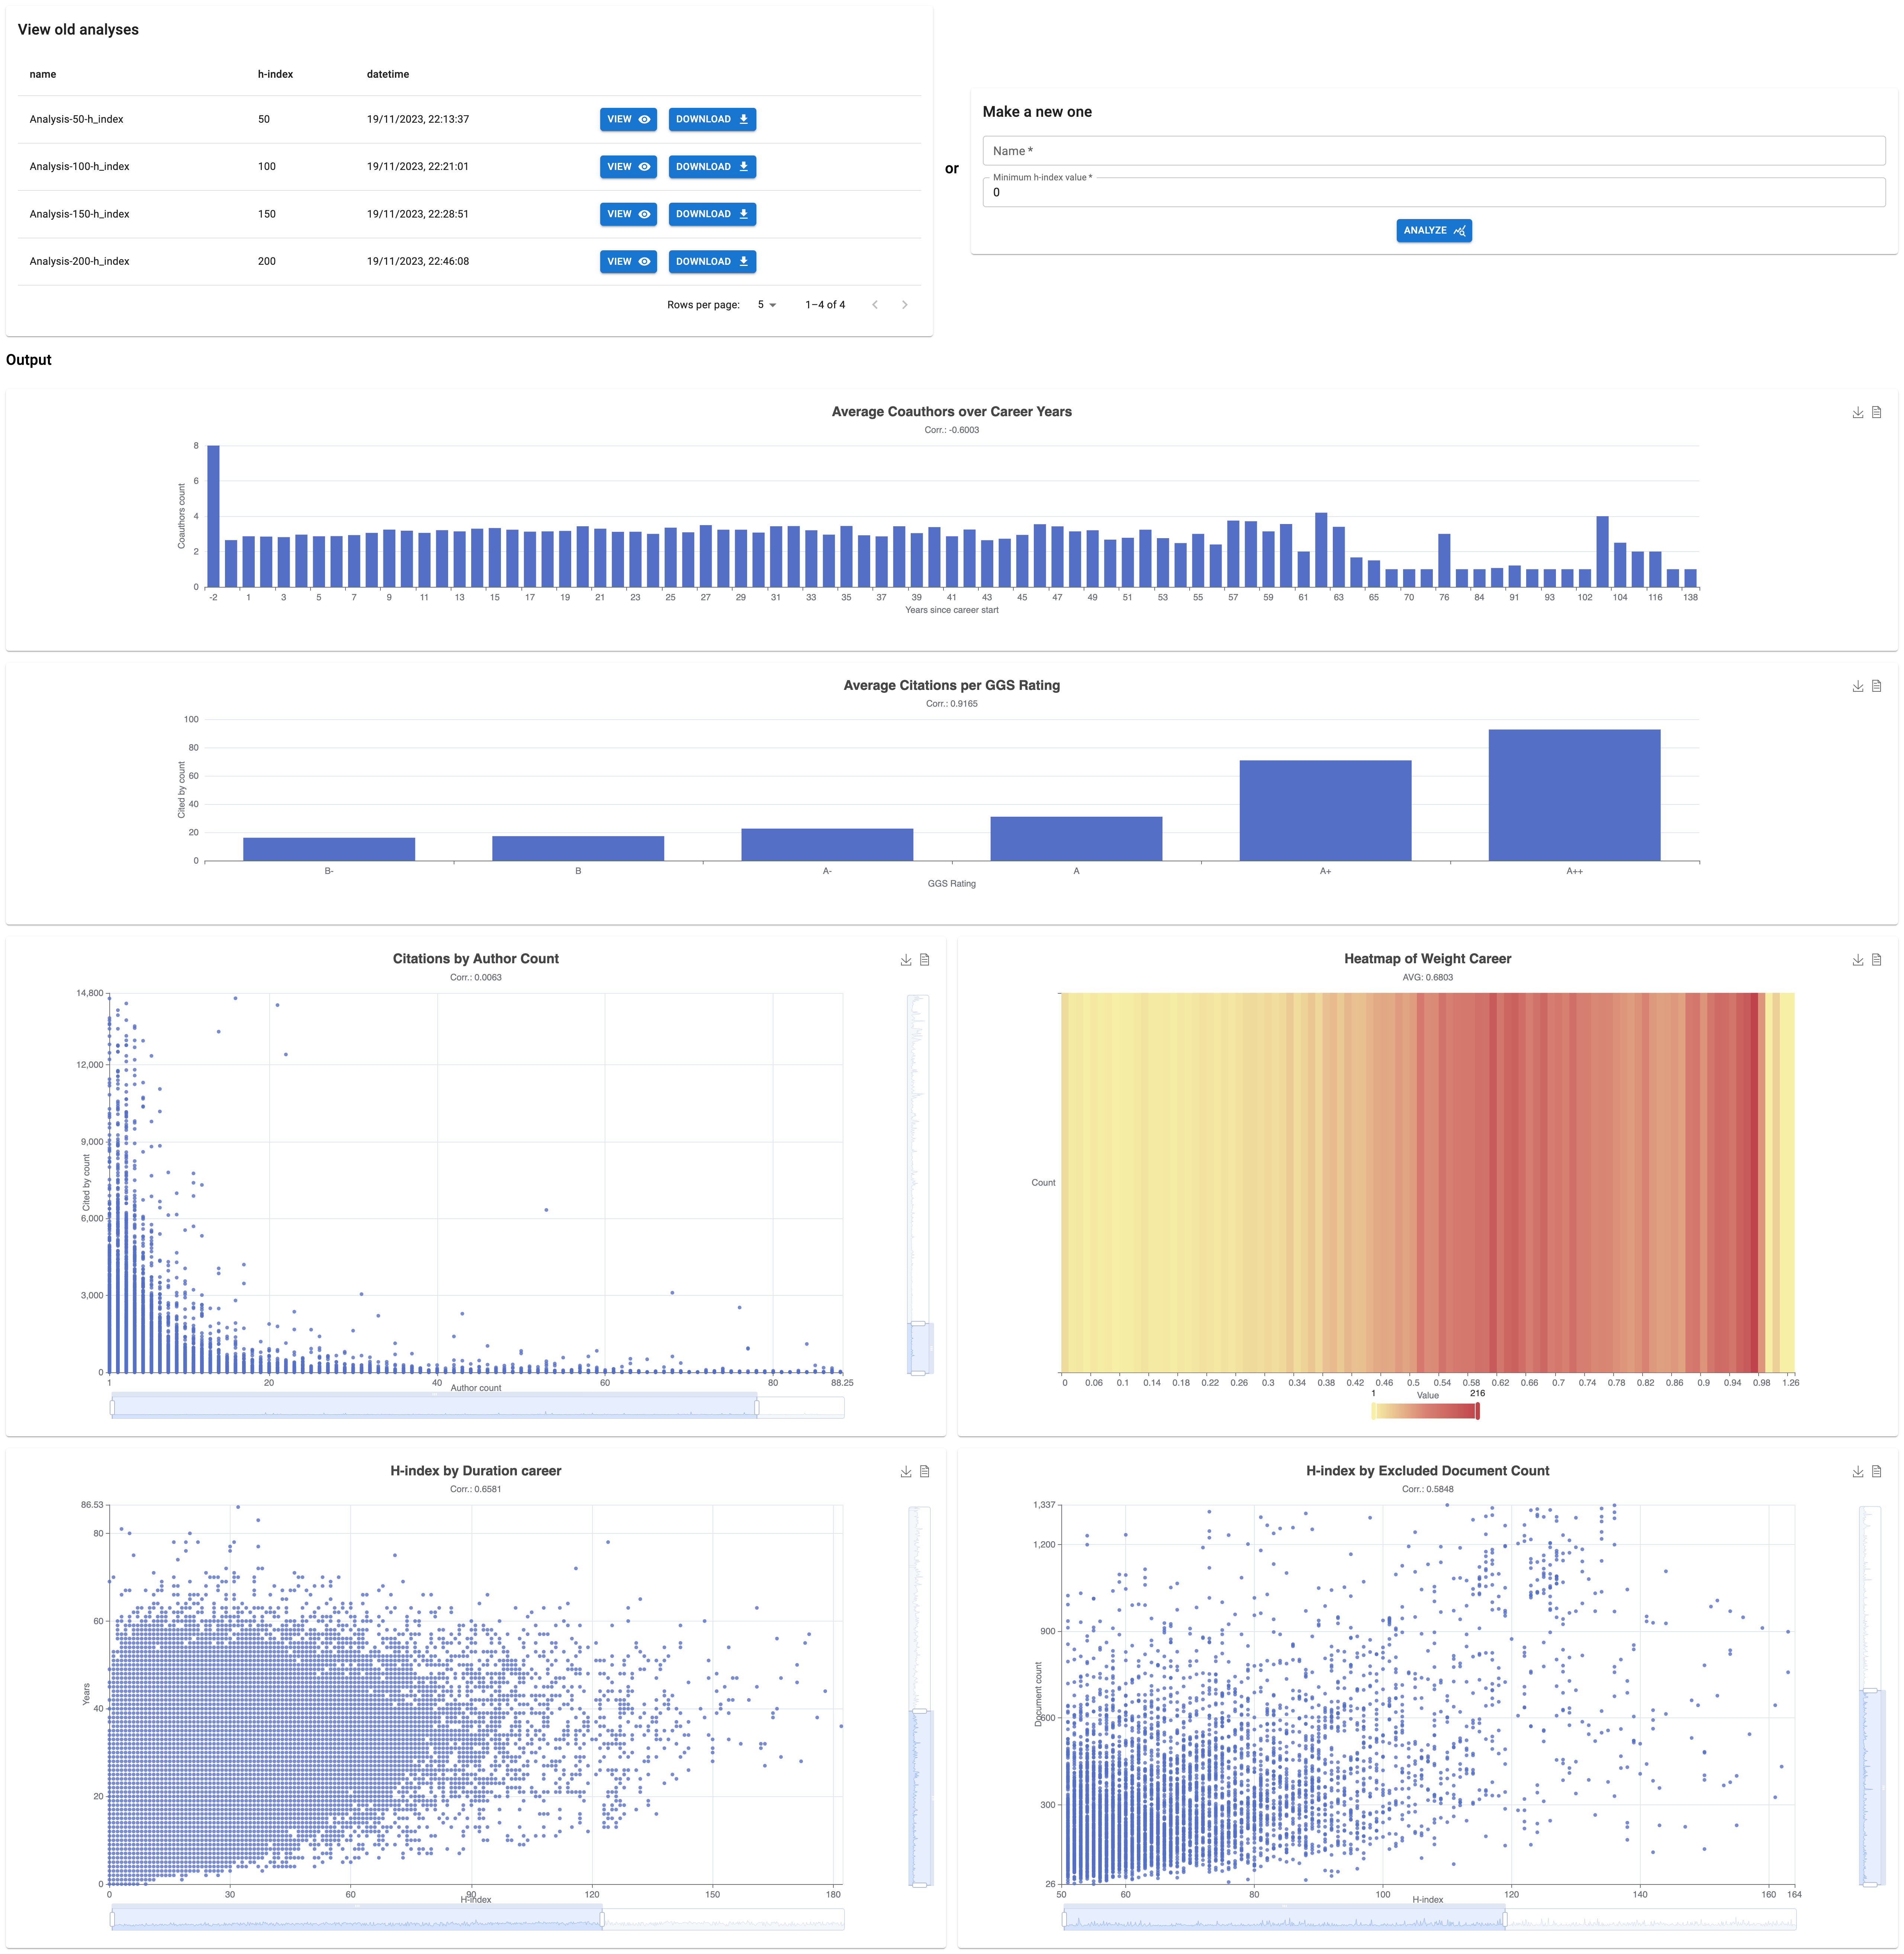
\includegraphics[width=0.9\textwidth]{images/dashboard.png}
    \caption{Dashboard}
    \label{fig:dashboard}
\end{figure}


I diagrammi sono stati accuratamente selezionati per adattarsi alle diverse nature dei dati: i grafici di dispersione offrono una visione dinamica delle variazioni e delle tendenze, i grafici a barre permettono un confronto immediato tra diverse categorie, e le mappe di calore espongono le relazioni complesse attraverso una gradazione cromatica. 
Ogni diagramma è scaricabile in formato vettoriale assicurando che la qualità delle immagini rimanga inalterata a prescindere dallo scaling, permettendo così una visualizzazione ottimale in ogni contesto, sia esso digitale o cartaceo.
Inoltre per i grafici a dispersione è stata aggiunta la possibilità di ingrandire determinate aree per visualizzare meglio zone con alte concentrazioni di dati.

Per completare l'offerta di strumenti a disposizione degli utenti, è stata introdotta una funzionalità di esportazione che permette di scaricare sia i dati delle analisi che i grafici corrispondenti in formato vettoriale, raccolti in un unico file .zip. Questo aspetto facilita notevolmente la distribuzione e la condivisione dei risultati, rendendo il processo di esportazione un'operazione semplice e veloce. La creazione dell'archivio compresso è resa possibile dall'impiego della libreria JSZip \cite{jszip}, come illustrato nel Codice~\ref{lst:export_archive_ts}.

\begin{lstfloat}
    \begin{lstlisting}[
    language=JavaScript,
    caption={Esportazioni dati e immagini},
    label={lst:export_archive_ts},
    breaklines=true,
    postbreak=\mbox{\textcolor{red}{$\hookrightarrow$}\space}
    ]
const exportData = (data: Analysis) => {
    const zip = new JSZip();
    const analysis = zip.folder('analysis');
    getAllEcharts()
    .forEach((instance: ECharts, index: number) => {
        let dataUrl = decodeURIComponent(instance.getDataURL());
        dataUrl = dataUrl.substring(dataUrl.indexOf(',') + 1);
        analysis?.file(`chart-${index}.svg`, dataUrl);
    });
    
    analysis?.file(
      `${data.name}.json`, 
      JSON.stringify(data)
    );
    
    zip.generateAsync({type:'blob'})
    .then(function(content) {
      saveAs(content, `${data.name}.zip`);
    });
};
    \end{lstlisting}
\end{lstfloat}


\chapter{Analisi dei dati e risultati}
\section{Dataset e hardware utilizzato}

Per evidenziare le capacità e le potenzialità del software sviluppato, sono state condotte diverse analisi esemplificative basate su un ampio volume di dati bibliografici. A tal fine, sono stati raccolti tutti gli articoli pubblicati nell'ambito ``Computer Science'' dal 1850 al 2022, per un totale di 8.2 milioni. Questo corpus, di dimensioni notevoli, riflette lo sviluppo storico e l'evoluzione dell'informatica. Nonostante ciò, a causa di restrizioni imposte dalle API per l'accesso ai dati, sono state raccolte informazioni complete su soli circa 460.000 autori, una porzione significativa, ma non completa, dei 6.6 milioni di autori totali in questo campo. Un riassunto dettagliato del dataset è presentato nella Tabella~\ref{tab:overview_dataset}.
Questo insieme di dati, sebbene non totalmente rappresentativo dell'intera comunità accademica in informatica, fornisce un quadro chiaro delle tendenze e delle evoluzioni tecnologiche che hanno segnato quasi due secoli di ricerca.

\begin{table}[ht]
    \centering
    \begin{tabular}{|l|r|r|}
        \hline
        \textbf{Collezione} & \textbf{Documenti}  & \textbf{Dimensione totale} \\
        \hline
        \texttt{collectionAuthors} & $466\cdot10^3$ su $6.6\cdot10^6$ &  5.15 GiB \\
        \hline
        \texttt{collectionAbstracts} & $8.2\cdot10^6$ & 17.47 GiB \\
        \hline
        \texttt{collectionAuthorsAggregate} & $466\cdot10^3$ & 17.66 GiB \\
        \hline
    \end{tabular}
    \caption{Panoramica dati scaricati per analisi}
    \label{tab:overview_dataset}
\end{table}

Le analisi sono state effettuate su un MacBook Pro equipaggiato con un chip M1 Pro e 16 GiB di memoria RAM, operante con il sistema operativo macOS versione 13.6 (22G120). Il processo analitico è stato gestito attraverso un ambiente Docker (v24.0.6), ottimizzato per sfruttare al meglio le risorse hardware disponibili. In particolare, il container Docker è stato configurato per utilizzare tutti i 10 core del dispositivo, allocando alla macchina virtuale 12 GiB di RAM e 3 GiB di memoria swap aggiuntiva.

\section{Analisi e grafici}
Al fine di testare approfonditamente il software sviluppato, è stata pianificata l'esecuzione di quattro diverse analisi, ciascuna con soglie distinte di $h$-index: 50, 100, 150 e 200. L'obiettivo di questa sperimentazione era duplice: in primo luogo, valutare il tempo di risposta del software in seguito alla chiamata dell'API, e in secondo luogo, analizzare le dimensioni del documento JSON fornito in risposta. Queste metriche sono cruciali per determinare sia l'efficienza operativa del software sia la sua capacità di gestire richieste di dati di varie grandezze. I risultati di queste analisi, che riflettono l'efficacia del software sotto diverse condizioni operative, sono riportati nella Tabella~\ref{tab:overview_metrics_performance}. Questi dati forniscono un'importante indicazione sulle prestazioni e l'affidabilità del sistema in scenari di utilizzo reali, offrendo un quadro chiaro dell'adattabilità e della robustezza del software.

\begin{table}[ht]
    \centering
    \begin{tabular}{|r|r|r|}
        \hline
        \textbf{$h$-index minimo} & \textbf{Tempo di risposta} & \textbf{Dimensione} \\
        \hline
        50 & 6.5 min & 2.1 MiB \\
        \hline
        100 & 4.8 min & 1.6 MiB \\
        \hline
        150 & 4.5 min & 1.5 MiB \\
        \hline
        200 & 4.7 min & 1.5 MiB \\
        \hline
    \end{tabular}
    \caption{Metriche di performance delle analisi}
    \label{tab:overview_metrics_performance}
\end{table}

Per il presente studio, sono stati selezionati i grafici relativi alle analisi con soglie di $h$-index pari a 50 e 150, considerate le più significative.

\begin{figure}[ht]
    \centering
    \begin{subfigure}{0.49\textwidth}
        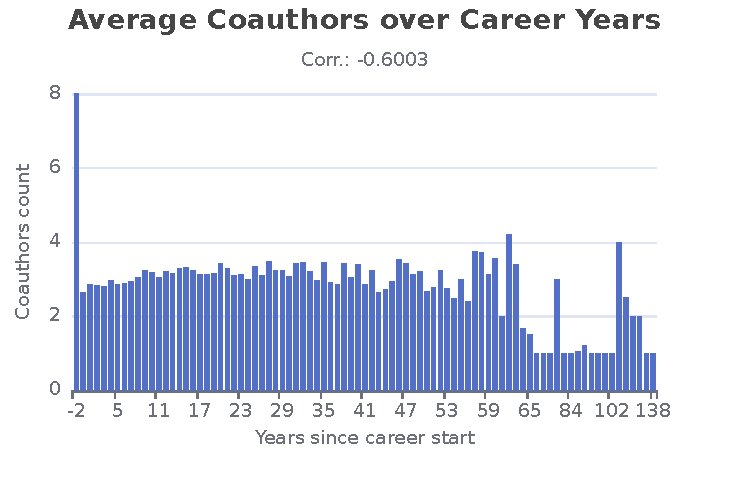
\includegraphics[width=\textwidth]{images/Average-Coauthors-over-Career-Years-50.pdf}
        \caption{Soglia 50}
        \label{fig:Average-Coauthors-over-Career-Years-50}
    \end{subfigure}
    \hfill
    \begin{subfigure}{0.49\textwidth}
        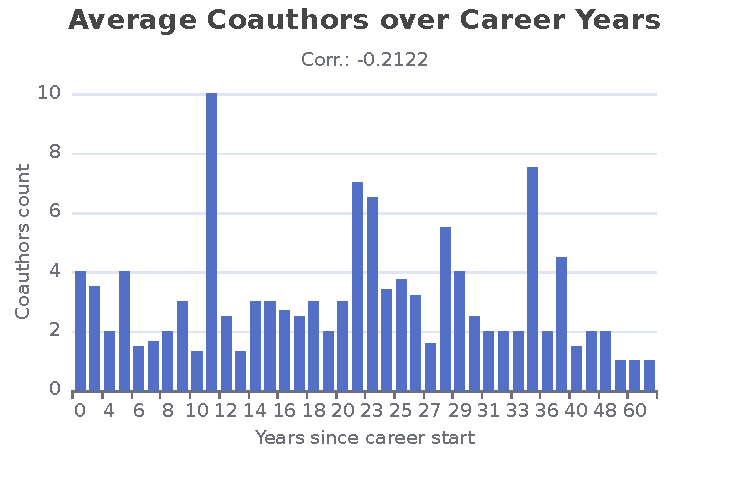
\includegraphics[width=\textwidth]{images/Average-Coauthors-over-Career-Years-150.pdf}
        \caption{Soglia 150}
        \label{fig:Average-Coauthors-over-Career-Years-150}
    \end{subfigure}        
    \caption{Grafici della variazione media dei coautori nel tempo}
    \label{fig:Average-Coauthors-over-Career-Years}
\end{figure}

Il confronto visualizzato in Figura~\ref{fig:Average-Coauthors-over-Career-Years} illustra l'evoluzione delle dinamiche di collaborazione tra i ricercatori nel corso della loro carriera. Dall'analisi emerge una tendenza generale alla riduzione del numero di coautori nel tempo. Interessante notare come questa tendenza sia meno marcata negli autori con un $h$-index più elevato, suggerendo che i ricercatori più affermati mantengano un livello di collaborazione più costante rispetto ai loro colleghi.

\begin{figure}[ht]
    \centering
    \begin{subfigure}{0.49\textwidth}
        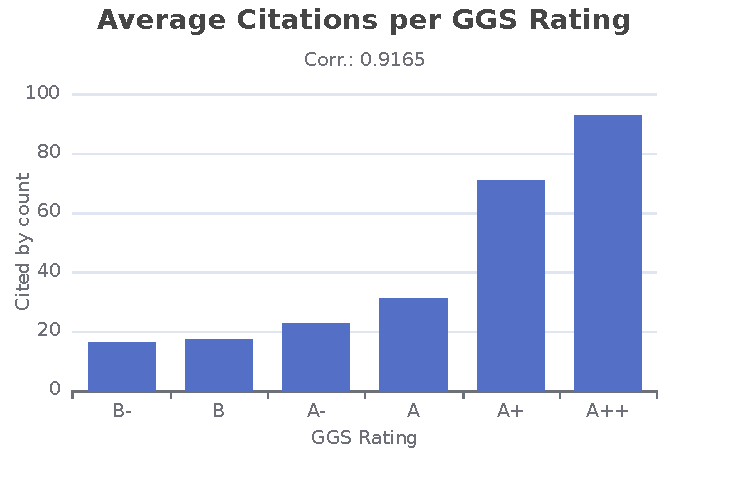
\includegraphics[width=\textwidth]{images/Average-Citations-per-GGS-Rating-50.pdf}
        \caption{Soglia 50}
        \label{fig:Average-Citations-per-GGS-Rating-50}
    \end{subfigure}
    \hfill
    \begin{subfigure}{0.49\textwidth}
        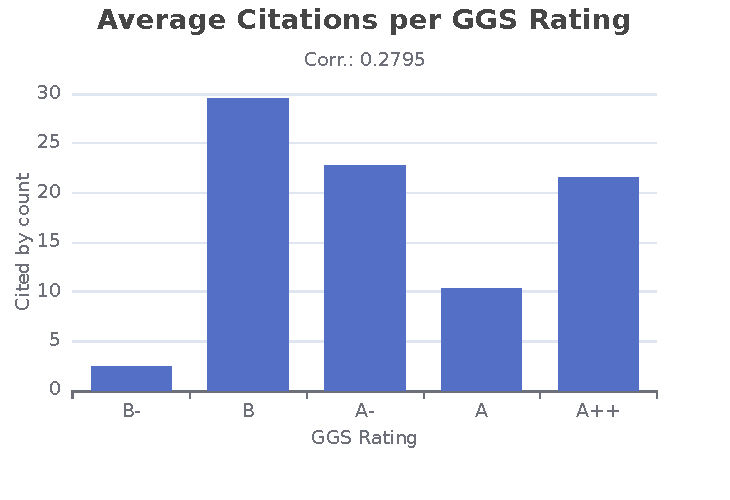
\includegraphics[width=\textwidth]{images/Average-Citations-per-GGS-Rating-150.pdf}
        \caption{Soglia 150}
        \label{fig:Average-Citations-per-GGS-Rating-150}
    \end{subfigure}        
    \caption{Grafici dell'impatto del rating di una conferenza sul numero di citazioni}
    \label{fig:Average-Citations-per-GGS-Rating}
\end{figure}

La Figura~\ref{fig:Average-Citations-per-GGS-Rating} illustra la relazione tra la classificazione delle conferenze informatiche e il numero medio di citazioni per articolo. È evidente che, per il gruppo con un $h$-index superiore a 50, esiste una forte relazione tra il prestigio del convegno e il numero di citazioni ricevute. Tuttavia, interessante notare come l'influenza della reputazione del congresso tenda a diminuire all'aumentare della soglia dell'$h$-index. Questo fenomeno suggerisce che, per gli autori con un elevato impatto nel mondo accademico, altri fattori oltre alla semplice reputazione del convegno possono avere un maggiore impatto sulle citazioni ricevute dai loro articoli.

\begin{figure}[ht]
    \centering
    \begin{subfigure}{0.49\textwidth}
        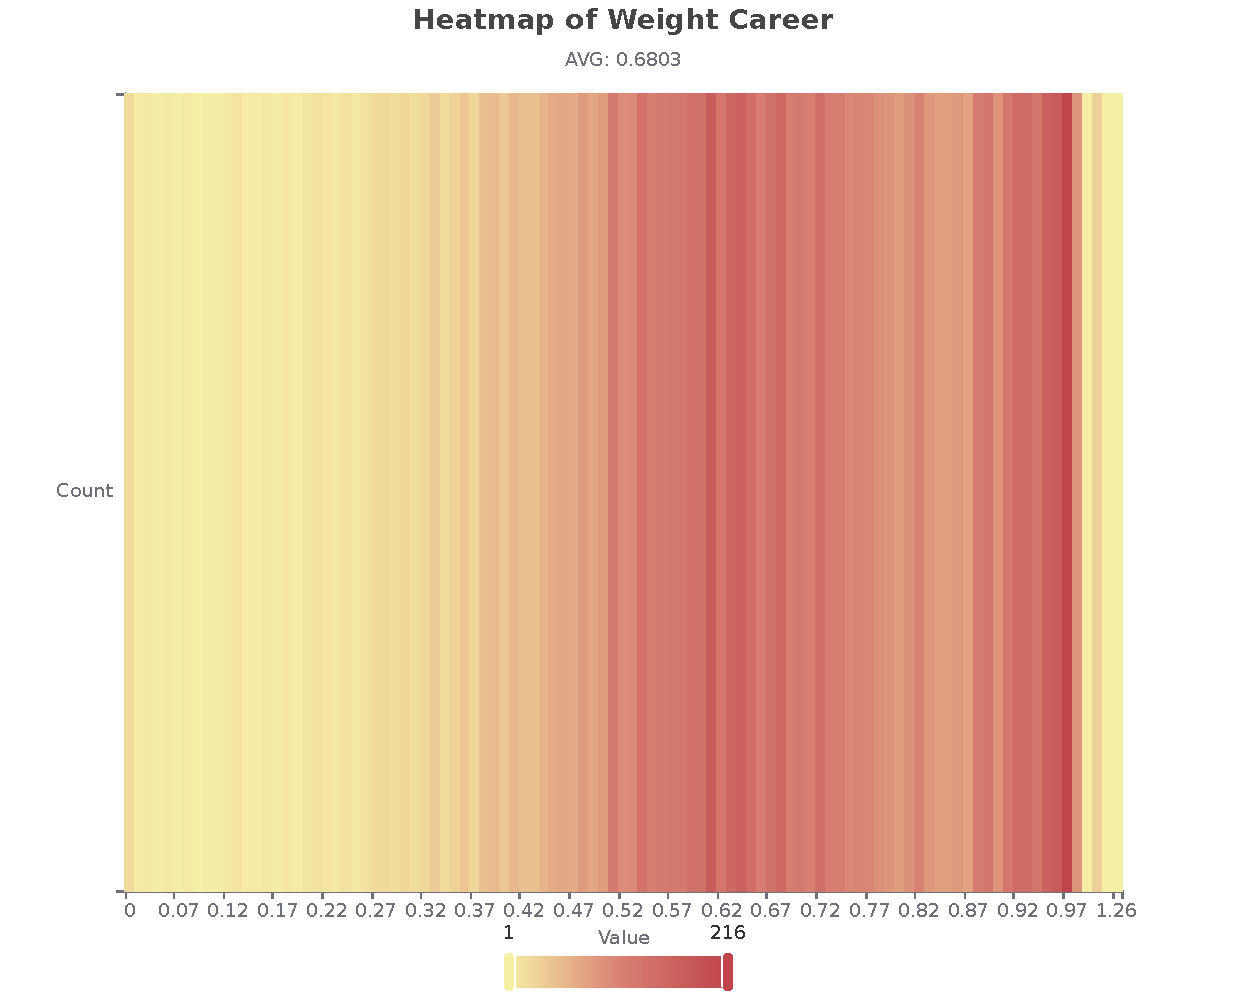
\includegraphics[width=\textwidth]{images/Heatmap-of-Weight-Career-50.pdf}
        \caption{Soglia 50}
        \label{fig:Heatmap-of-Weight-Career-50}
    \end{subfigure}
    \hfill
    \begin{subfigure}{0.49\textwidth}
        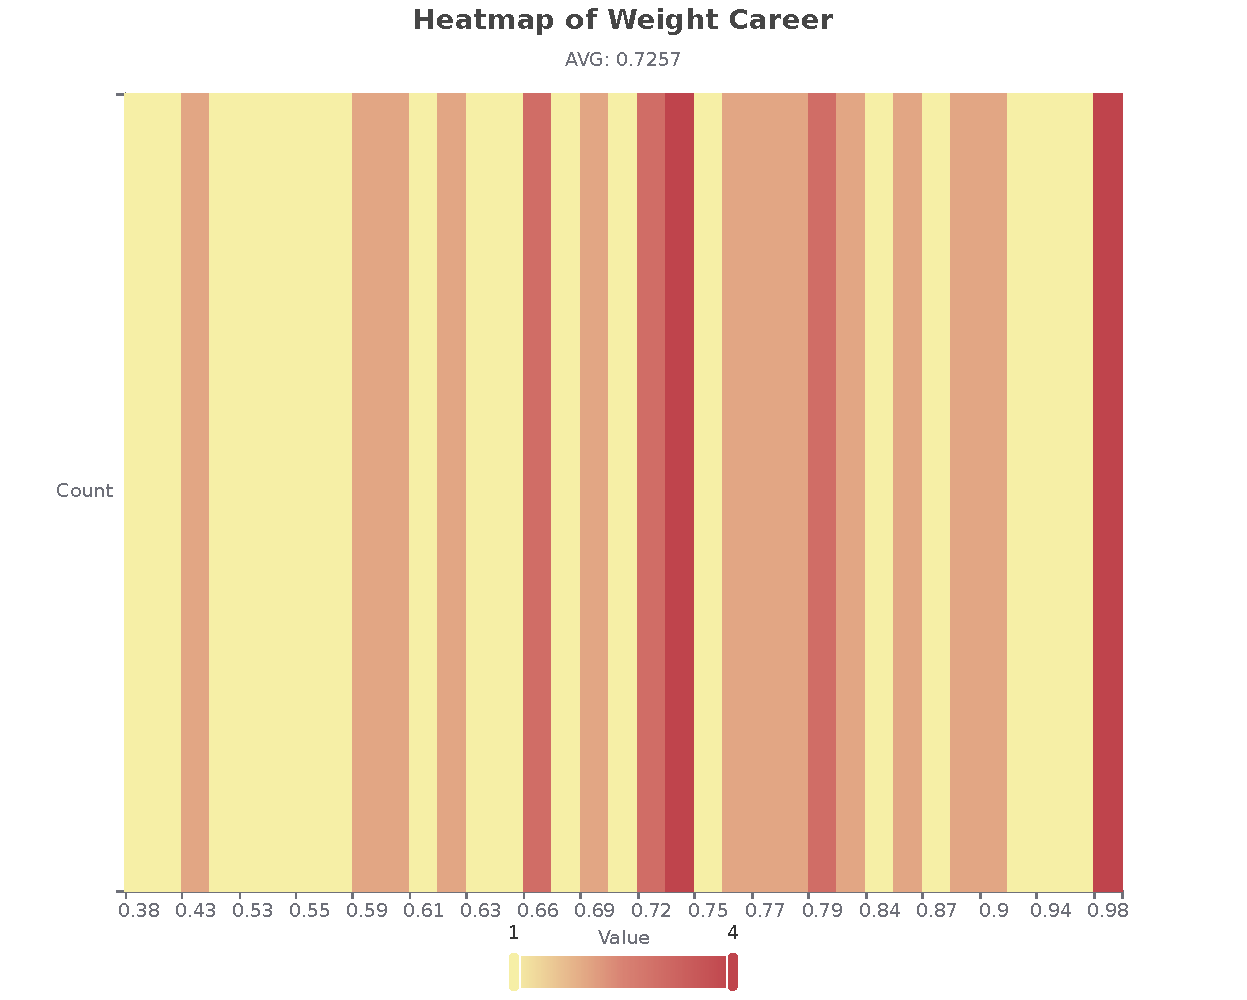
\includegraphics[width=\textwidth]{images/Heatmap-of-Weight-Career-150.pdf}
        \caption{Soglia 150}
        \label{fig:Heatmap-of-Weight-Career-150}
    \end{subfigure}        
    \caption{Grafici dell'analisi del momento di pubblicazione di articoli influenti sull'$h$-index}
    \label{fig:Heatmap-of-Weight-Career}
\end{figure}

L'analisi visualizzata nella Figura~\ref{fig:Heatmap-of-Weight-Career} mette in luce un aspetto relativo alla carriera accademica degli autori: in media, gli articoli che influenzano maggiormente l'$h$-index tendono a essere pubblicati dopo la metà della loro carriera, questa tendenza si mantiene con un impatto maggiore per tutta la seconda metà della loro attività accademica, suggerendo che il periodo più produttivo e influente per molti ricercatori si verifica nella fase matura della loro carriera.

\begin{figure}[ht]
    \centering
    \begin{subfigure}{0.49\textwidth}
        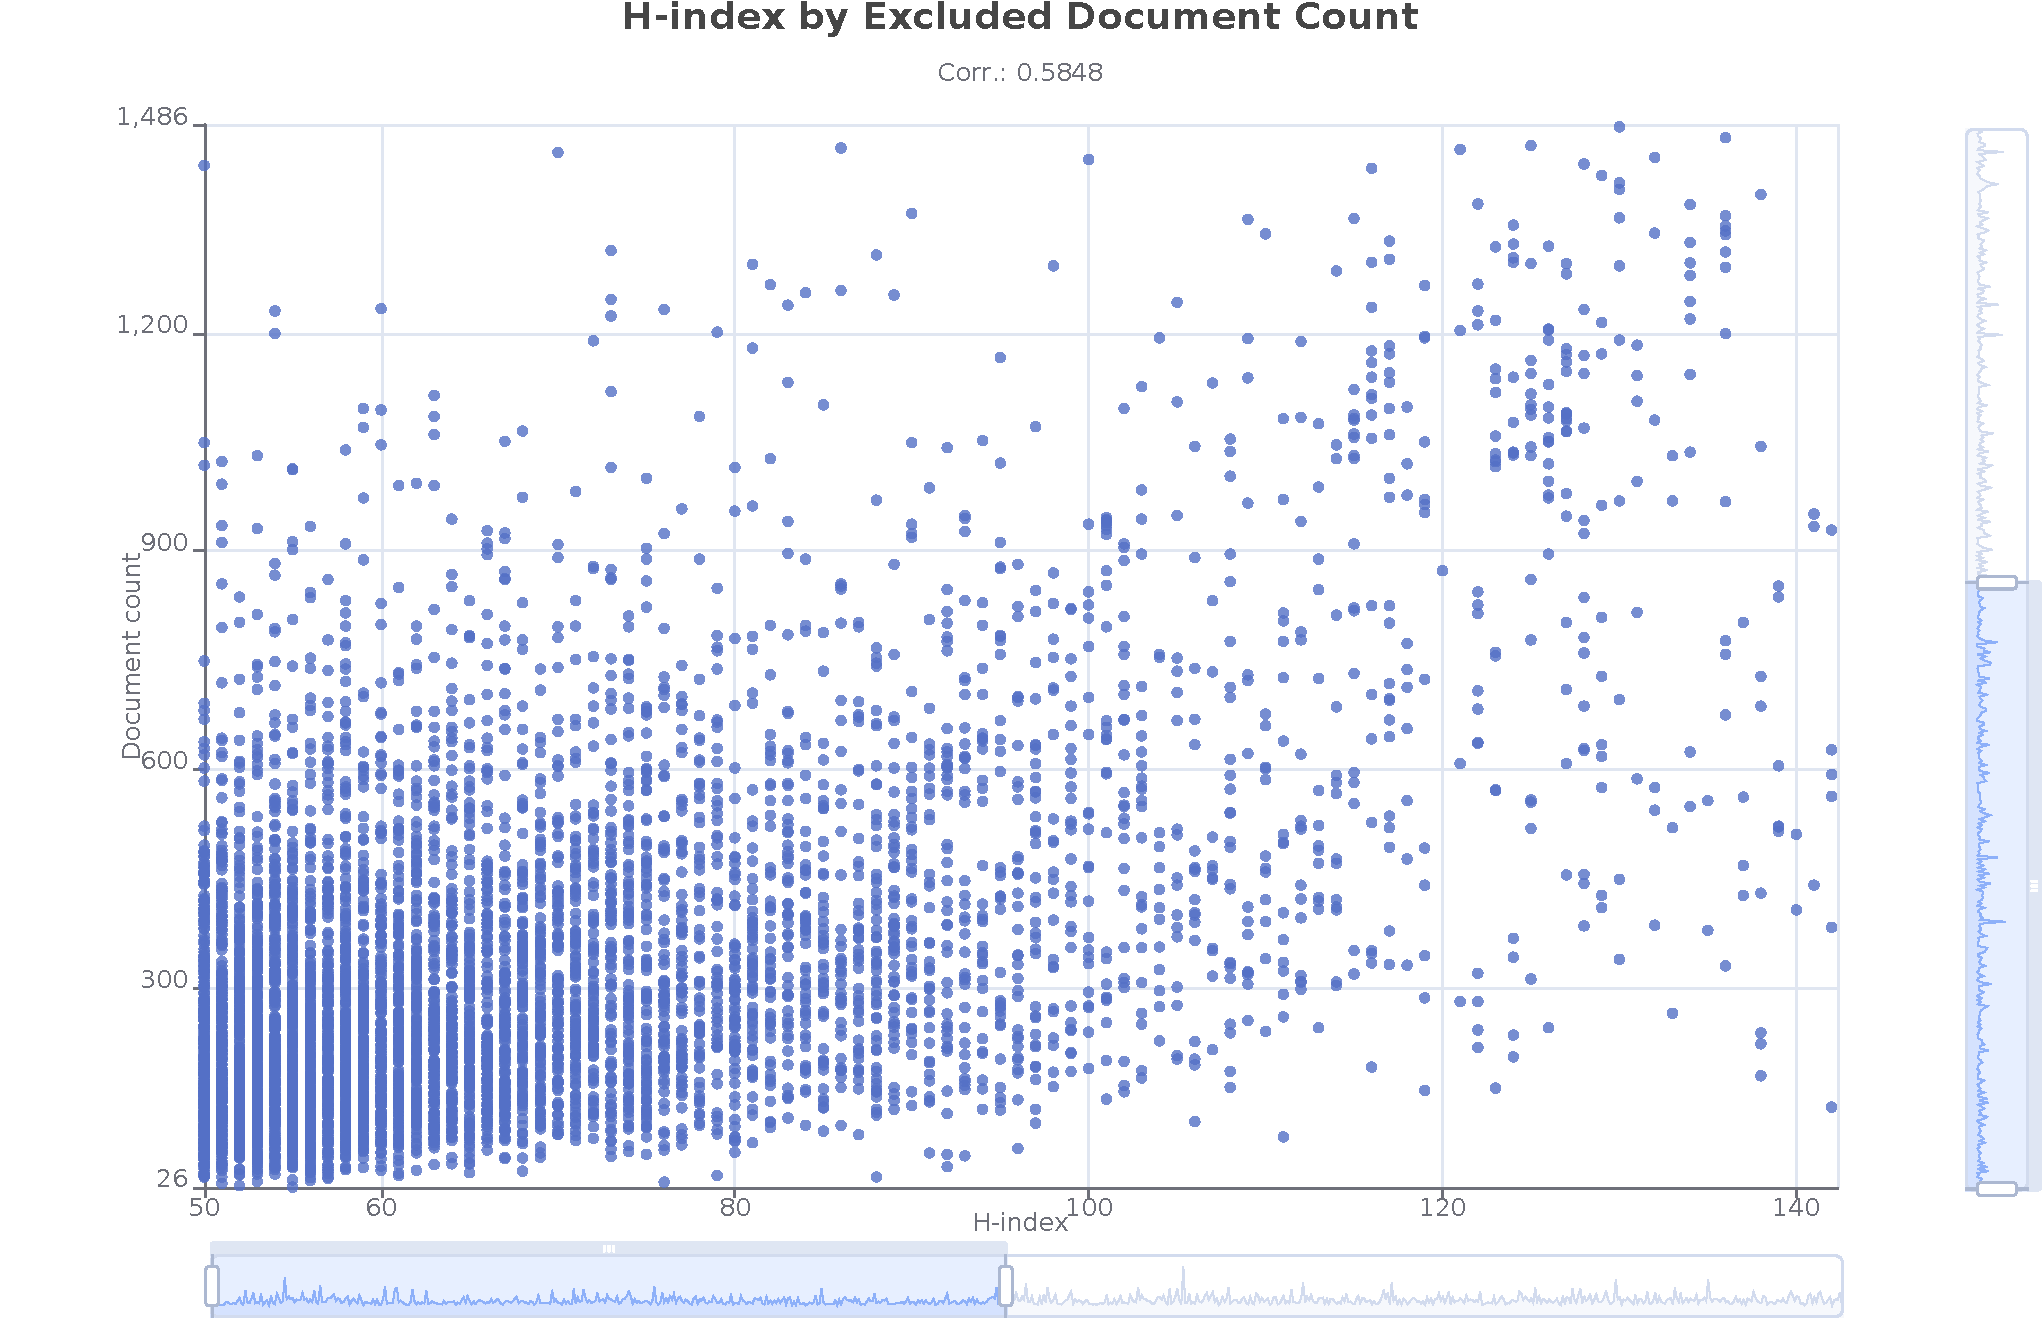
\includegraphics[width=\textwidth]{images/H-index-by-Excluded-Document-Count-50.pdf}
        \caption{Soglia 50}
        \label{fig:H-index-by-Excluded-Document-Count-50}
    \end{subfigure}
    \hfill
    \begin{subfigure}{0.49\textwidth}
        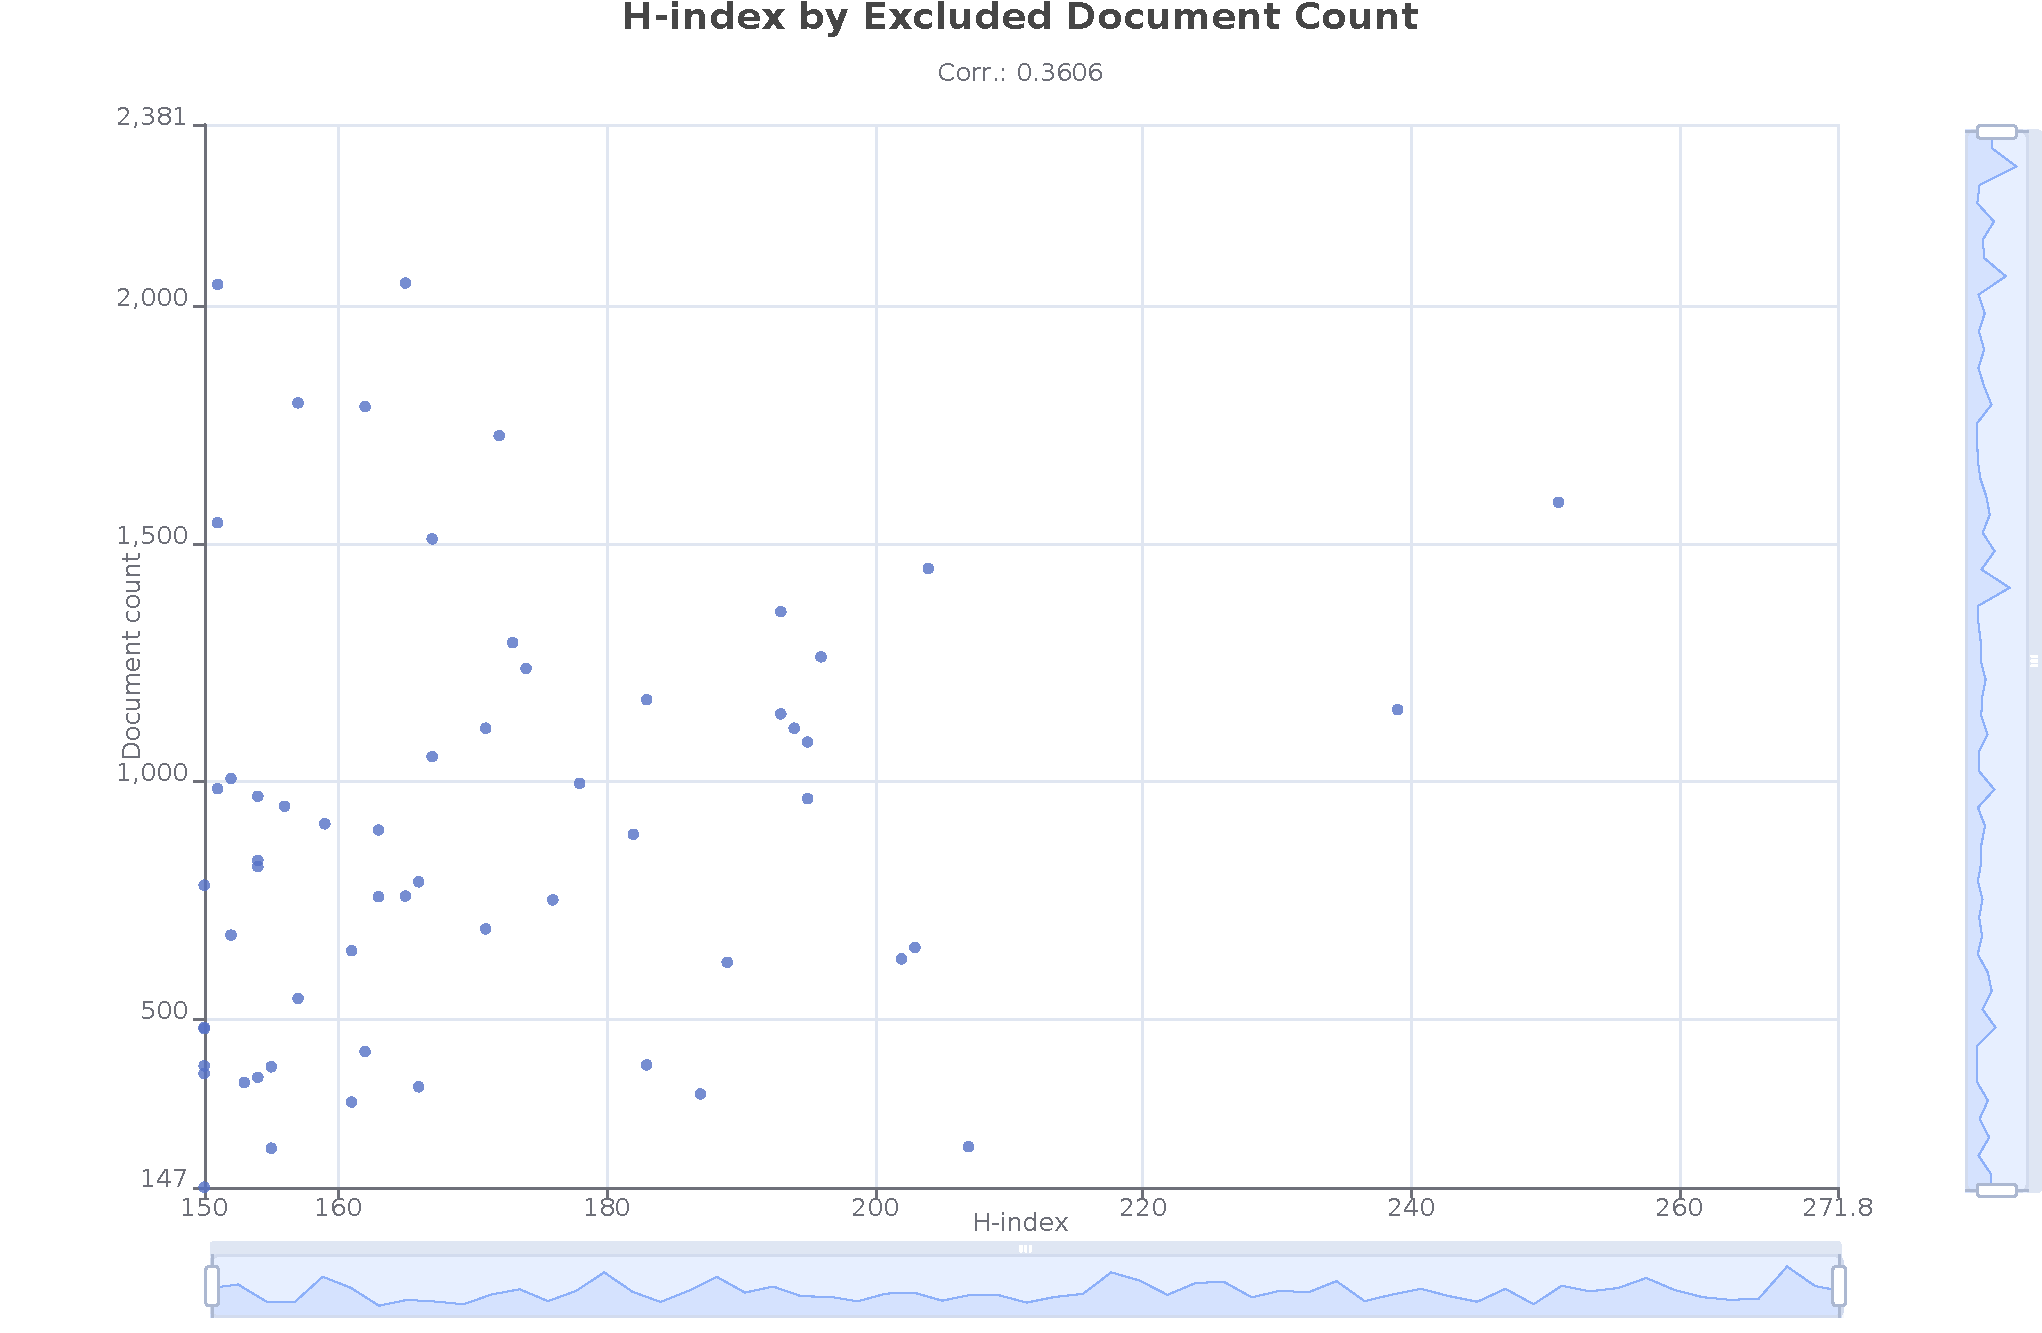
\includegraphics[width=\textwidth]{images/H-index-by-Excluded-Document-Count-150.pdf}
        \caption{Soglia 150}
        \label{fig:H-index-by-Excluded-Document-Count-150}
    \end{subfigure}        
    \caption{Grafico della correlazione tra $h$-index e articoli esclusi}
    \label{fig:H-index-by-Excluded-Document-Count}
\end{figure}

L'analisi della correlazione tra l'$h$-index degli autori e il numero di documenti esclusi dal calcolo di quest'ultimo è descritta in Figura~\ref{fig:H-index-by-Excluded-Document-Count}. Si osserva una correlazione moderata, che implica che gli autori con un numero maggiore di lavori tendono generalmente ad avere un valore più elevato. Questo suggerisce che una produttività accademica più alta può portare a un indice di impatto più alto, anche se non tutti i documenti contribuiscono direttamente all'$h$-index.

La relazione tra il conteggio degli autori di un articolo e il numero di citazioni ricevute è mostrato in Figura~\ref{fig:Citations-by-Author-Count}. Il grafico mostra una correlazione molto debole  tra queste due variabili, suggerendo che il numero di ricercatori di un paper non ha un impatto significativo sul numero di citazioni ricevute.

\begin{figure}[ht]
    \centering
    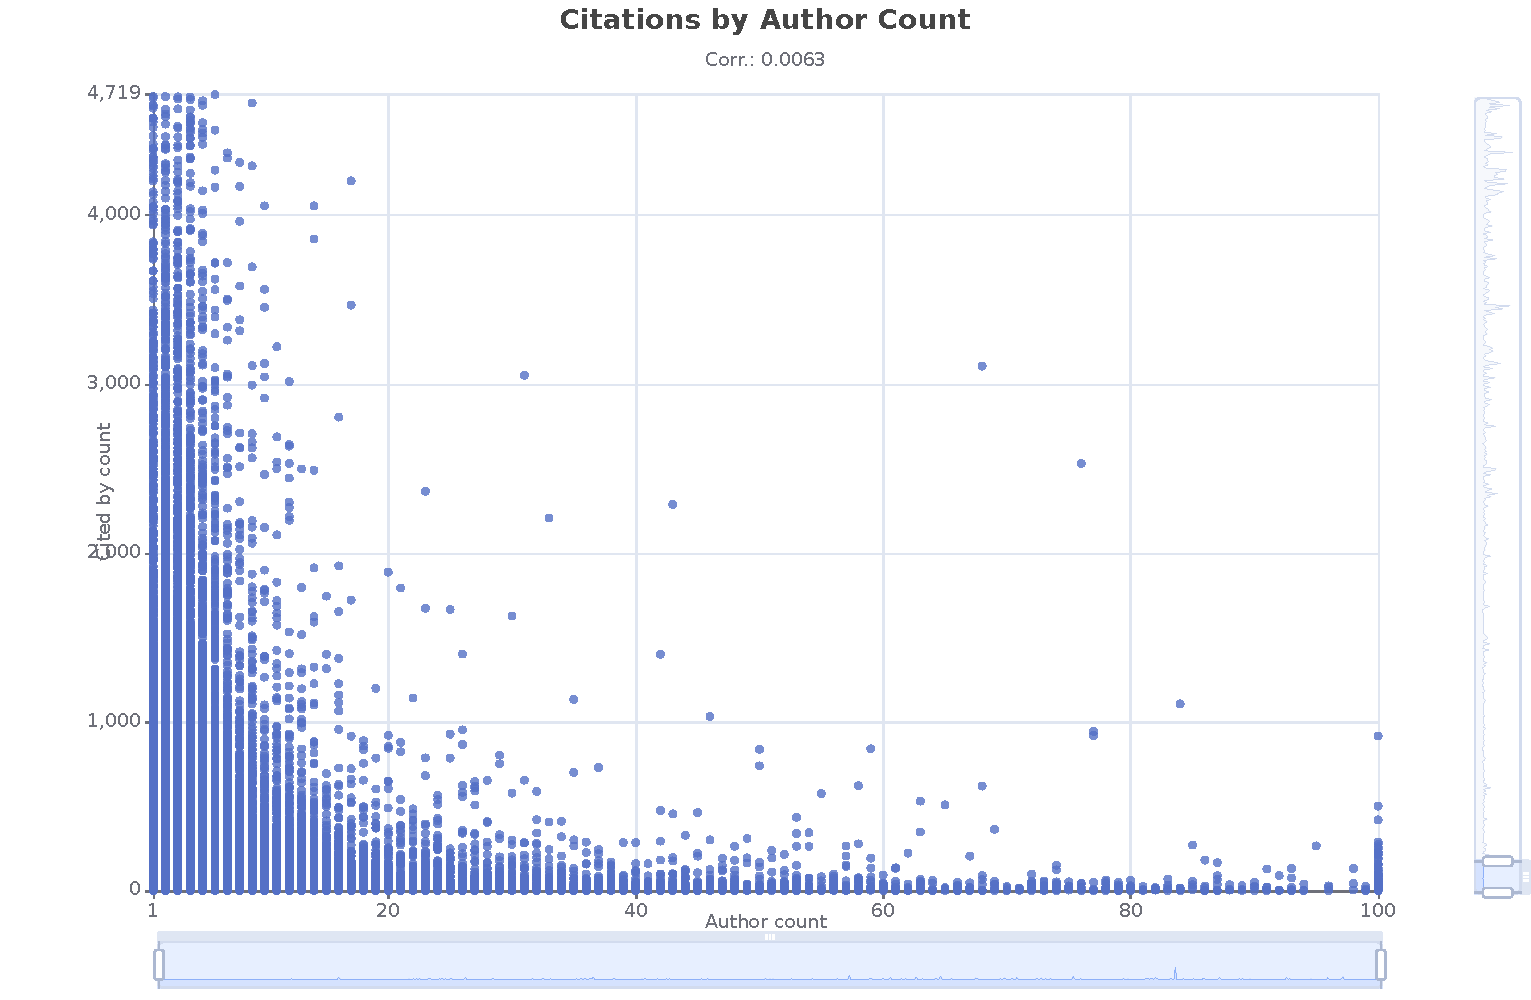
\includegraphics[width=.7\textwidth]{images/Citations-by-Author-Count.pdf}
    \caption{Grafico dell'impatto del numero di coautori sulle citazioni}
    \label{fig:Citations-by-Author-Count}
\end{figure}

La Figura~\ref{fig:H-index-by-Duration-career} evidenzia una correlazione sostanziale tra la durata della carriera di un autore e il suo $h$-index indicando che generalmente un valore più alto corrisponde a una carriera più lunga nel campo della ricerca. La relazione tra questi due fattori sottolinea l'importanza dell'esperienza e del tempo dedicato in ambito accademico nell'incrementare l'accumulo di citazioni e, di conseguenza, nell'ottenere un $h$-index elevato.

\begin{figure}[ht]
    \centering
    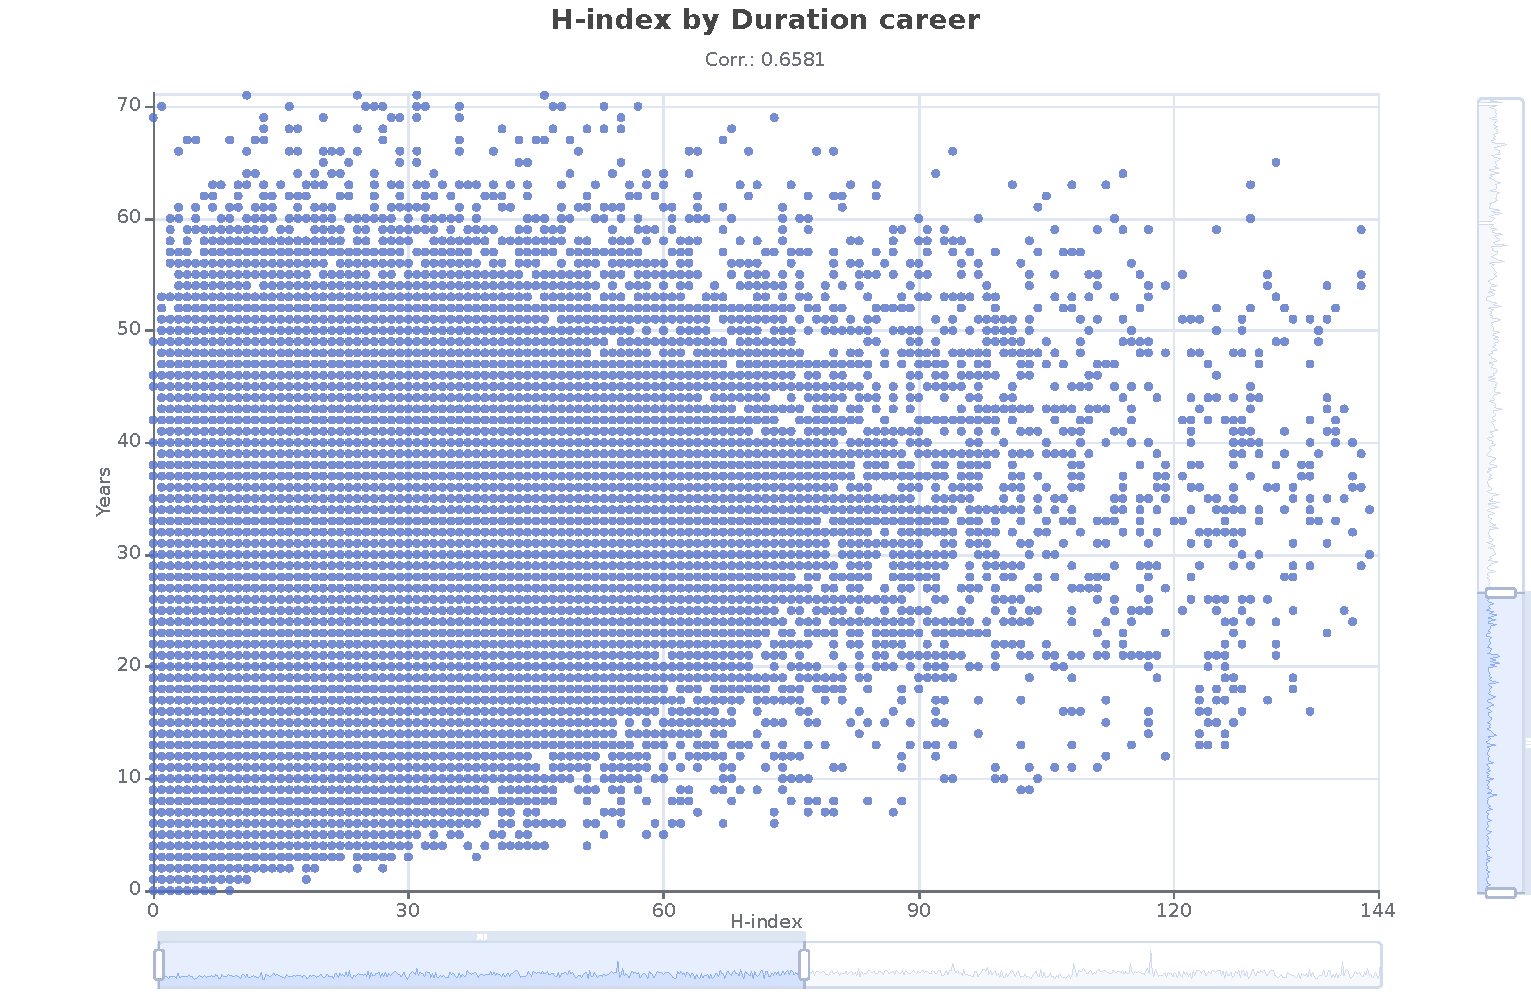
\includegraphics[width=.7\textwidth]{images/H-index-by-Duration-career.pdf}
    \caption{Correlazione tra $h$-index e durata della carriera}
    \label{fig:H-index-by-Duration-career}
\end{figure}


\section{Commenti e riflessioni sui risultati}
Esaminando nel loro insieme i risultati dei grafici, emerge un quadro complesso e dettagliato della carriera accademica, caratterizzato da dinamiche interessanti.
Questi dati rivelano che, indipendentemente dal livello di $h$-index, esistono trend comuni ma anche differenze significative nelle traiettorie accademiche. Per esempio, la tendenza alla riduzione delle collaborazioni nel corso della carriera è meno evidente negli autori con un $h$-index molto elevato. Questo suggerisce che i ricercatori più affermati, forse a causa della loro consolidata reputazione e rete di contatti, mantengono un livello di collaborazione elevato e stabile.

Inoltre, l'influenza della reputazione delle conferenze sul numero di citazioni ricevute tende a diminuire all'aumentare dell'$h$-index, ciò potrebbe indicare che, per i ricercatori di alto livello, la qualità e l'originalità della ricerca diventano più importanti del prestigio del convegno per ottenere riconoscimenti.

L'analisi sull'età dei contributi significativi per l'indice bibliometrico suggerisce che i ricercatori più esperti tendono a produrre lavori di impatto maggiore nella fase matura della loro carriera, forse grazie a una maggiore profondità di conoscenza e a reti di collaborazione ben sviluppate.

Infine, la correlazione tra la durata della carriera e l'$h$-index enfatizza l'importanza dell'esperienza prolungata e dell'impegno costante nella ricerca. I ricercatori con carriere più lunghe non solo hanno più tempo per pubblicare e accumulare citazioni, ma anche per sviluppare e affinare le loro competenze di ricerca.

In conclusione, questi grafici illustrano l'importanza di una visione a lungo termine nella carriera accademica, dove la costruzione di reti solide, la scelta strategica delle conferenze, e l'approfondimento continuo delle competenze di ricerca sono cruciali per raggiungere e mantenere un alto livello di impatto e riconoscimento nel campo accademico.
\chapter{Conclusioni}

\section{Limitazioni dello studio}
Durante la progettazione, lo sviluppo e il successivo utilizzo del software, sono emerse diverse limitazioni che meritano un'attenta considerazione:

\begin{enumerate}
    \item \textbf{Restrizioni delle API}: le restrizioni imposte dalle API di Scopus, come il limite alle richieste e il numero massimo di chiavi, hanno limitato l'ampiezza e la profondità dell'analisi.

    \item \textbf{Limitazioni dell'$h$-index}: l'$h$-index, pur essendo un utile indicatore bibliometrico, ha le sue critiche e limitazioni \cite{ding2020exploring}. Non fornisce un quadro completo dell'impatto e dell'influenza di un autore ed è soggetto a variazioni a seconda della piattaforma bibliografica utilizzata e del fenomeno dell’autocitazionismo.

    \item \textbf{Aggiornamento dei dati}: la rapidità con cui si evolvono le pubblicazioni e le citazioni nel campo accademico e la possibilità di aggiornare e correggere le informazioni presenti sulla piattaforma Scopus rendono i dati raccolti rapidamente obsoleti influenzando la rilevanza e l'attualità delle analisi eseguite.
    
    \item \textbf{Analisi quantitativa e qualitativa}: la focalizzazione su analisi quantitative potrebbe tralasciare aspetti qualitativi importanti della ricerca, come l'influenza culturale, l'impatto sociale o l'importanza teorica, che non sono catturabili attraverso metodi bibliometrici.

\end{enumerate}

Queste sono le maggiori restrizioni riscontrate durante lo svolgimento del presente lavoro, portando a considerare evoluzione future differenti trattate nel prossimo paragrafo.

\section{Sviluppi futuri per il software}
Considerando le limitazioni evidenziate in precedenza, si propone un'evoluzione del progetto che differisce dall'attuale percorso. Per superare i vincoli imposti dalle API, si suggerisce di orientare l'analisi verso gruppi più specifici implementando funzionalità che consentano la selezione e l'analisi di autori associati a particolari università, campi di studio o stati, fornendo inoltre la possibilità di combinare questi filtri. Tale approccio potrebbe offrire analisi più mirate e dettagliate, contribuendo a una comprensione più profonda delle dinamiche accademiche specifiche.
Un'altra possibile evoluzione del progetto, sempre per mitigare i limiti imposti dalle API, includerebbe la funzionalità di permettere agli utenti di caricare un elenco specifico di autori da analizzare, attraverso l'upload di un file, o di selezionarli tramite una barra di ricerca. Questo miglioramento offrirebbe una maggiore personalizzazione nell'analisi, consentendo agli utenti di concentrarsi su gruppi di autori di loro interesse specifico.

Inoltre, le migliorie proposte offrirebbero la possibilità di creare rapidamente degli snapshot di specifici gruppi di ricerca, consentendo di osservare e analizzare la loro evoluzione nel tempo.
Per andare oltre le limitazioni dell'$h$-index, si potrebbe sviluppare un'analisi focalizzata sulle citazioni e sulla loro correlazione con autori appartenenti alla stessa università o alla stessa area geografica. Questo tipo di analisi permetterebbe di esplorare le dinamiche di collaborazione e di influenza all'interno di specifici ambienti accademici o comunità geografiche.

Infine, un'ulteriore evoluzione utile per semplificare e rendere più intuitiva l'usabilità del sistema potrebbe essere l'integrazione delle funzionalità di raccolta e aggregazione dati nell'interfaccia utilizzata per la creazione, gestione e visualizzazione delle analisi, eliminando la necessità di alternare tra la linea di comando e la dashboard.

\section{Commenti finali}
Questo lavoro ha raggiunto con successo gli obiettivi prefissati, stabilendo una base solida nel campo dell'analisi bibliometrica di gruppo attraverso lo sviluppo del presente software. L'applicazione non solo soddisfa le esigenze iniziali di acquisizione e analisi dei dati bibliometrici, ma introduce anche un'interfaccia utente intuitiva che semplifica l'accesso e l'esplorazione di queste analisi. Tuttavia, è chiaro che esistono ampi margini di manovra per il miglioramento poiché il potenziale per rendere il software e il flusso di lavoro più semplice è evidente e le possibilità di evoluzione sono molteplici. In definitiva, il lavoro svolto pone le basi per sviluppi futuri che possono rendere lo strumento ancora più prezioso per la comunità accademica e scientifica.
\chapter*{Ringraziamenti}

Desidero ringraziare UniBG Seclab per aver fornito il modello LaTeX \cite{thesis-template} utilizzato durante la stesura di questa tesi.

\nocite{*}
\printbibliography[heading=bibintoc]

\end{document}
